A partir de los datos de los casos penales, pudimos
construir la red de Grupos de Pertenencia. En esta red, se eliminan los nodos de aquellas personas cuyos roles no sean referidos a actores delictivos, como ser: denunciantes, víctimas, damnificados, etc. En la Figura \ref{fig:grafocompleto} se muestra una visualización de la red. En la misma se puede observar un grafo compuesto de las 200 personas con más Casos Penales registrados en el Sistema de Gestión Coirón (con los siguientes criterios: involucradas en al menos un caso con rol de imputado, sospechoso o denunciado; se incluyen personas fallecidas, menores y personas jurídicas). Se visualizan además en la figura todas las relaciones que existen entre esas 200 personas y sus grupos de pertenencia.

También hemos incluido estadísticas resumidas en la \ref{tab:EstadisticasResumidas}, en donde se pueden ver la cantidad de nodos y vértices totales con los que cuenta el dataset utilizado, como así también otros parámetros interesantes de analizar para el estudio de redes sociales.

Al analizar la composición de la red obtenida podemos observar las relaciones que existen entre los nodos y como se "equilibra" el grafo, haciendo que aquellos nodos con pocas o nulas relaciones queden en la periferia de la gráfica. Sumado a ello también es apreciable la medida de centralidad de aquellos nodos que son rodeados por sus relacionados.

Una aproximación más clara para denotar la medida de centralidad puede verse reflejada en la Figura \ref{fig:grafoTop10}, en donde se visualiza sólo las 10 personas con más Casos y sus grupos de pertenencia. Claramente esos 10 nodos principales quedan rodeados de sus grupos de pertenencia y se pueden observar transitividades entre ellos a través de nodos que conforman parte del grupo de pertenencia de más de un nodo principal.
\todo{hablar un poco de la distribución de datos}

\todo{script de SQL para generar la tabla 2(cantidad de nodos, vertices, ver si puedo calcular transitividad, y otros parámetros}


\begin{figure}
	\centering
	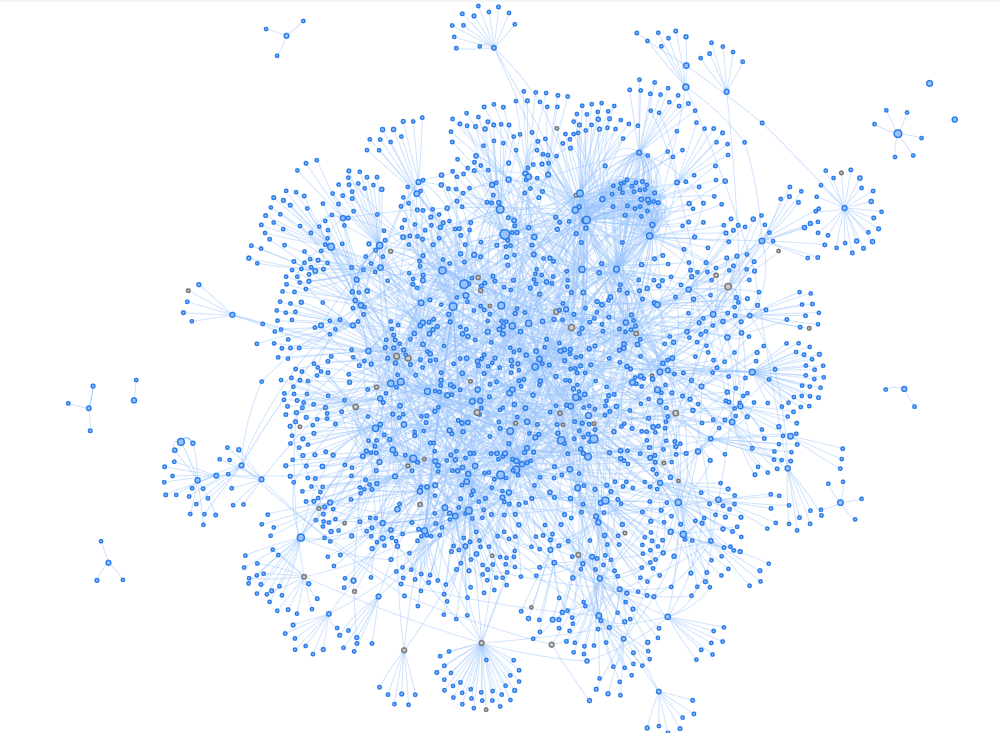
\includegraphics[width=\textwidth]{grafo-200-completo.png}
	\caption{Grafo obtenido del Sistema Coirón. 200 personas con más casos y sus relaciones (con los siguientes criterios: involucradas en al menos un caso con rol de imputado, sospechoso o denunciado; se incluyen personas fallecidas, menores y personas jurídicas)} 
	\label{fig:grafocompleto}
\end{figure}

\begin{table}
	\caption{Estadísticas resumidas de la DB}
	\label{tab:EstadisticasResumidas}
\end{table}

\begin{figure}
	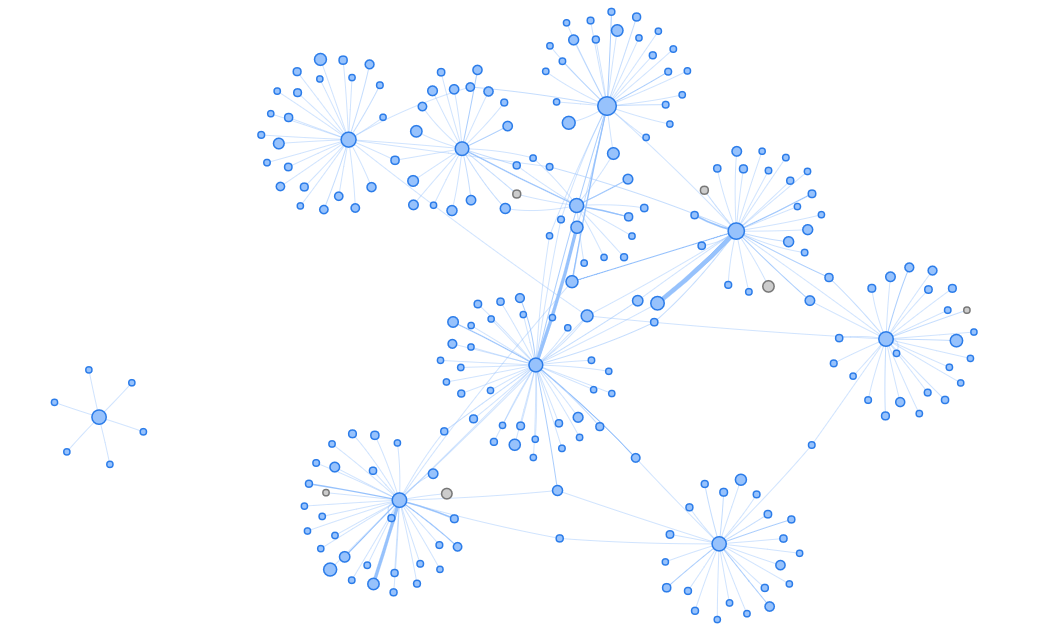
\includegraphics[width=\textwidth]{grafo-10-completo.png}
	\caption{10 personas con más casos en Coirón, con sus relaciones} 
	\label{fig:grafoTop10}
\end{figure}

\subsubsection{Centralidad} Please place your acknowledgments at

\subsubsection{Transitividad} Please place your acknowledgments at

